\documentclass{beamer}
\usetheme{metropolis}           % Use metropolis theme
\usepackage{blindtext}
\usepackage{enumitem}
\usepackage{chemformula}




\title{Phosphorus Release from Eroded Soil in the Aquatic Systems}
\date{\today}
\author{Antti-Jussi Kallio}
\institute{University of Helsinki}
\begin{document}
  \maketitle
  \section{Phosphorus cycle}
  \begin{frame}{Erosion}
    \begin{itemize}
    \item[*] Erosion control measures are applied all over the world, in many cases to protect the soil itself, or to reduce off-site impacts  
    \item[*] Does controlling soil erosion inhibit aquatic eutrophication (rehev{\"o}ityminen)?
      \begin{itemize}
        \item[-] The main interest of our study
        \item[-] We study the mineralization pathways of \ch{Fe}, which is coupled to \ch{C}, \ch{S} and \ch{P} cycling.
        \item[-] The amount of \ch{C}, \ch{S}, aerobic vs anaerobic.
      \end{itemize}
    \end{itemize}
  \end{frame}
  \begin{frame}{Possible effects of eroded soil on eutrophication}
    \begin{itemize}
      \item[*] \small{(The following summarize applies to estuary (murtovesi), or any \ch{SO4} rich recipient.)}
      \item[*] If the estuary receives a high input of \ch{Fe} oxides and a modest level of dissolved \ch{P}, we may see 		  moderate levels of eutrophication.
      \item[*] The settling flux has a low \ch{C}/\ch{Fe} ratio and the sediment is mainly in \ch{Fe} reduction state.
      \begin{itemize}
        \item[-] As a result the estuary may respond to erosion control because the \ch{P} concentrations are not maintained by strong \ch{P} release from the sediment due to coupled cycling of \ch{P} and \ch{Fe}. 
	  \end{itemize}
	  \item[*] The biotic fauna releases \ch{Fe} and \ch{P} from the oxides which then react with \ch{O2} in the aerobic estuary.
	  \begin{itemize}
		\item[-] No \ch{P} release from sediment to the aquatic system, keeps the "ferrous wheel" spinning.	
	  \end{itemize}	        
    \end{itemize}
  \end{frame}
  
  
  \begin{frame}{Possible effects of eroded soil on eutrophication}
    \begin{figure}
      \centering
      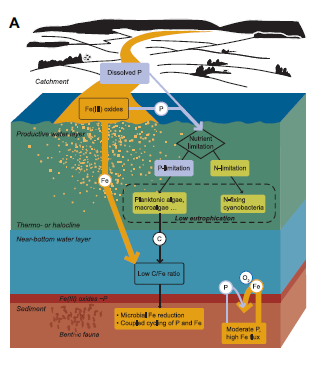
\includegraphics[scale=0.55]{../Kuvat/eutrophication_A.png}  
      \caption{\footnotesize{\ch{Fe} and \ch{P} cycle in aerobic estuary}}   
    \end{figure}
  \end{frame}
  
  \begin{frame}{Possible effects of eroded soil on eutrophication}
  \begin{itemize}
    \item[*] If erosion control takes place, typically dissolved \ch{P} increases as we reduce the input of \ch{Fe} oxides.
    \item[*] Increased bioavailable \ch{P} triggers algal (lev{\"a}) production, which increases the flux of organic \ch{C} to the sediment surface $\rightarrow$ \ch{SO4} reduction becomes important
    \item[*] The lowered flux of \ch{Fe} oxides means higher \ch{C}/\ch{Fe} ratio.
    \item[*] When \ch{SO4} reduction rates increase, more of the sediment \ch{Fe} is transformed to non-sorptive \ch{Fe} sulfides $\rightarrow$ massive release of \ch{Fe}-bound \ch{P} stored in sediments. 
    \item[*] Now the highly eutrophic estuary can show extensive cyonobacterial booms and benthic fauna may decrease.      
  \end{itemize}
  \end{frame}
  
  \begin{frame}{Possible effects of eroded soil on eutrophication}
  \begin{itemize}
    \item[*] The \ch{Fe} and \ch{P} cycle is affected by hydromorphology and chemistry of the receiving body of water.
    \begin{itemize}
      \item[-] In deep systems the organic \ch{C} is largely mineralized, so it does not effect the benthic processes.
      \item[-] The depth also affect sediment accumulation areas.
      \item[-] The lack of \ch{O2} affect the sediment state by affecting the mineralization and preventing the re-oxidization of \ch{Fe}(II).  
    \end{itemize}
    \item[*] The level of \ch{SO4} in the sediment also plays a crucial role.
    \item[*] The net effect of soil erosion on eutrophication depends on the balance between labile soil \ch{P} and the lowering of benthic \ch{P} release caused by \ch{Fe} oxides.
  \end{itemize}
  \end{frame}
  
  \begin{frame}{Possible effects of eroded soil on eutrophication}
    \begin{figure}
      \centering
      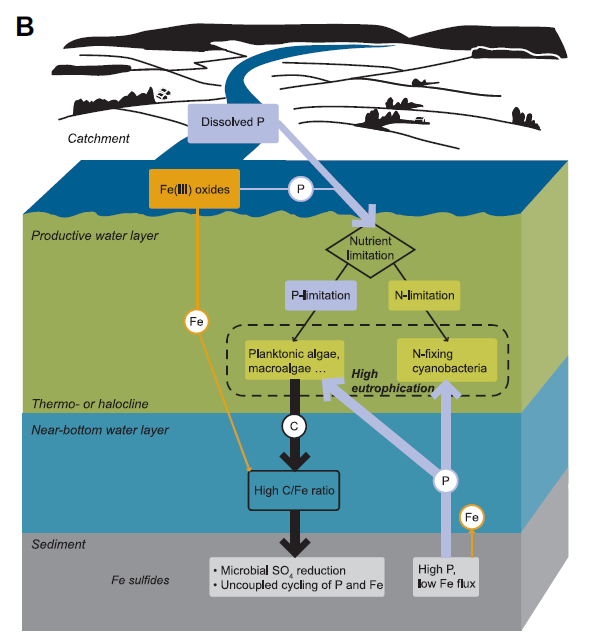
\includegraphics[scale=0.31]{../Kuvat/eutrophication_B.png}  
      \caption{\footnotesize{\ch{Fe} and \ch{P} cycle in anaerobic estuary}}   
    \end{figure}
  \end{frame}
  
  \begin{frame}{Points of interest}
  \begin{itemize}
    \item[*] The assumptions stated above need to be verified. The sediment processes are not well known. 
    \item[*] We need to gain information about the changes in mineralization of soil during the processes stated above in the molecular level.
  \end{itemize}
  \end{frame}
  
  \section{X-ray Absorption Spectroscopy}
  \begin{frame}{A small description of XAS}
  \begin{itemize}
    \item[*] X-ray absorption spectroscopy studies how x-rays are absorbed by an atom near and above its core-level binding energies.
    \item[*] When an X-ray is absorbed by an atom, core-level (K, L, M) electron is ejected (photoelectron). The atom is left in an exited state with empty electronic level.
    \item[*] The exited core-hole is relaxed, a higher level electron fills the empty space and a fluorescence x-ray or auger electron is emitted.
    \item[*] When discussing x-ray absorption, we are primarily concerned with the absorption coefficient $\mu$, which gives the probability that x-rays will be absorbed according to Beer's Law:   
  \end{itemize}
  \begin{equation}
  I=I_0e^{-\mu t} \rightarrow \mu(E)=\ln{\frac{I_0}{I_t}}
  \end{equation}
  \end{frame}
  
  \begin{frame}{A small description of XAS}
  \begin{columns}
    \begin{column}{0.5\textwidth}
    	  \begin{figure}
    	    \centering
    	    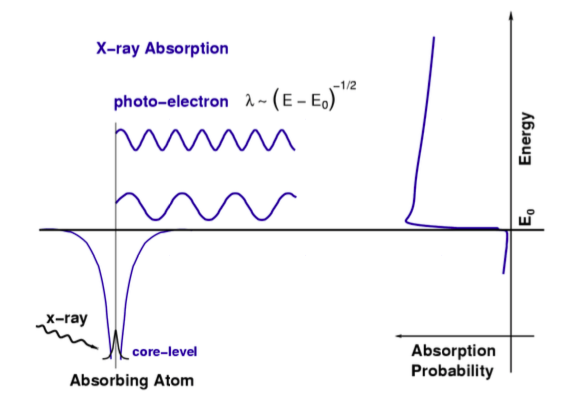
\includegraphics[width=1.2\textwidth]{../Kuvat/absorption1.png}
    	  \end{figure}
    \end{column}
    
    \begin{column}{0.5\textwidth}
      \begin{itemize}
        \item[*] \footnotesize{An incident x-ray of energy $E$ is absorbed, destroying a core-electron binding energy $E_0$, and emitting a photoelectron with kinetic energy $(E-E_0)$. The core state is eventually filled.} 
        \item[*] \footnotesize{When the incident x-ray energy is larger than the binding energy, there is a sharp increase in absorption}
        \item[*] \footnotesize{For an isolated atom, $\mu(E)$ has a sharp step at the core-level binding energy and is a smooth function of energy above the edge.}
      \end{itemize}
    \end{column}
  \end{columns}
  \end{frame}
  
  \begin{frame}{A small description of XAS}
  \begin{columns}
    \begin{column}{0.5\textwidth}
    	  \begin{figure}
    	    \centering
    	    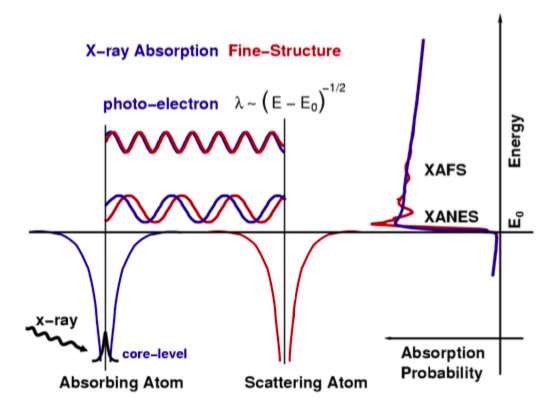
\includegraphics[width=1.2\textwidth]{../Kuvat/absorption2.png}
    	  \end{figure}
    \end{column}
    
    \begin{column}{0.5\textwidth}
      \begin{itemize}
        \item[*] \footnotesize{The ejected photoelectron can scatter from neighbouring atoms. $R$ is related to $\lambda$ and there is a phase shift associated with the scattering event. Thus outgoing and scattered waves interfere.} 
        \item[*] \footnotesize{The scattering photoelectron wave function interferes with itself. $\mu(E)$ depends on the density of states of the absorbing atom.}
        \item[*] \footnotesize{This interference at the absorbing atom will vary with energy, causing the oscillations with $\mu(E)$.}
      \end{itemize}
    \end{column}
  \end{columns}
  \end{frame}
  
  \begin{frame}{A small description of XAS}
  \begin{itemize}
    \item[*] XAS spectrum is typically divided into two regimes: XANES and EXAFS
    \begin{itemize}
      \item[-] XANES is strongly sensitive to formal oxidation state and coordination chemistry of the absorbing atom.
      \item[-] EXAFS is used to determine the distances, coordination number, and species of the neighbours of the absorbing atom.  
    \end{itemize}
    \item[*] Some benefits of XAS:
    \begin{itemize}
      \item[-] Element specific.
      \item[-] Many experimental techniques and sample conditions available.
    \end{itemize}
  \end{itemize}
  \end{frame}
  
  \begin{frame}{HelXAS}
  \begin{itemize}
    \item[*] In our experiment we are using XAS instrument called HelXAS, which can be found from the x-ray lab at the second floor. 
    \item[*] The instrument consists of three main components, x-ray tube, monochromator and detector. These components are motorised and follow the Rowland circle geometry.
    \item[*] Each monochromator crystal has a specific crystal orientation, so that we get the wanted wavelength according to Bragg's law:   
  \end{itemize}
  \begin{equation}
  2d_{hkl}sin\theta=n\lambda
  \end{equation}
  \begin{itemize}
    \item[*] Energy can be tuned around the edge by changing $\theta$
  \end{itemize}
  \end{frame}
  \begin{frame}{Measurement preparations}
  \begin{itemize}
    \item[*] The soil is mixed with sea water (from Seili and artificial), and \ch{C} and \ch{S} levels are varied.
    \item[*] To simulate anaerobic environment, we need an air tight sample environment and preferably a sample rotation to speed up the measurements.
    \item[*] The samples in a liquid phase needs to be tested
  \end{itemize}
  \end{frame}
  \section{Some early results}
  \begin{frame}{Dry soil samples}
  \begin{figure}
    \centering
    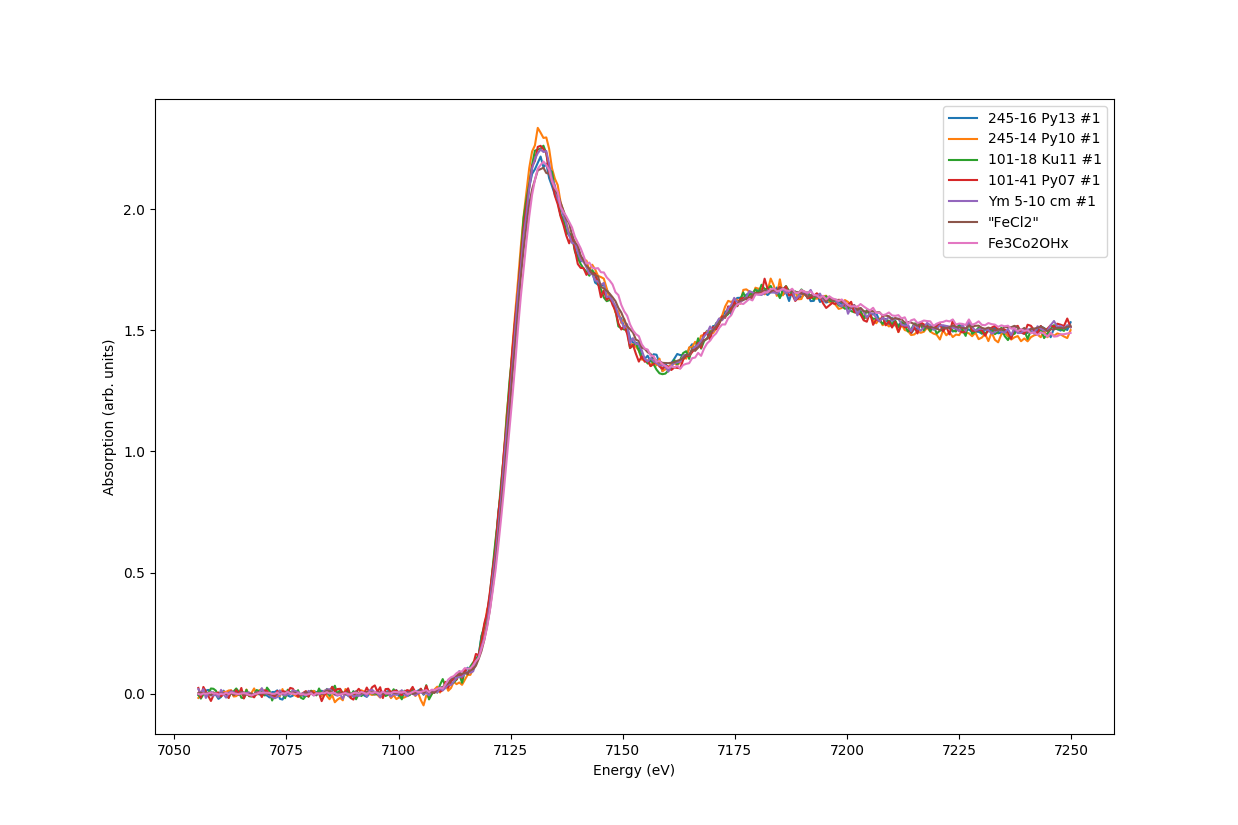
\includegraphics[width=0.9\textwidth]{../Kuvat/Dry_Soil_Samples1.png}
    \caption{Absorption spectrum of dry soil samples before incubation.}
  \end{figure}  
  \end{frame}
  
  \begin{frame}{Dry soil samples}
  \begin{figure}
    \centering
    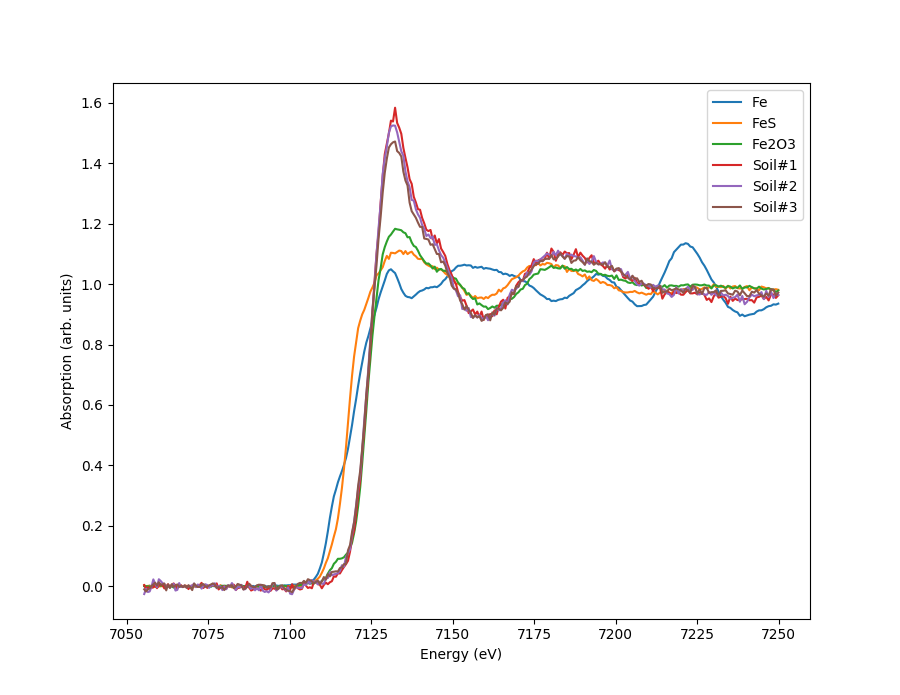
\includegraphics[width=0.8\textwidth]{../Kuvat/ferefplus123.png}
    \caption{Absorption spectrum of test soil sample and some reference materials.}
  \end{figure}  
  \end{frame}
  
  \begin{frame}{Wet aerobic soil mixed with sea water}
  \begin{itemize}
    \item[*] X-rays cause water molecules to break and release free \ch{O} radicals. Water "boils".
    \item[*] If sample places in front of the x-ray tube, all the water is gone in less than an hour. 
    \item[*] New sample environment allows to do measurement in front of the detector $\rightarrow$ much lower intensity and hopefully less radiation damage.
  \end{itemize}
  \end{frame}
  
  \begin{frame}{References}
  \begin{thebibliography}{9}
  \beamertemplatebookbibitems
  \bibitem{Soil erosion}
  Petri Ekholm, Jouni Lehtoranta.
  \textit{Does control of soil erosion inhibit aquatic eutrophication}.
  Journal of Environmental Management 93 (2012) 140-146.

  \beamertemplatebookbibitems
  \bibitem{Labile carbon}
  Lehtoranta J., Ekholm P., Wahlström S., Tallberg P., Uusitalo R.
  \textit{Labile organic carbon regulates phosphorus release from eroded soil transported into anaerobic coastal system}.
  Ambio 2015, 44(Suppl. 2) 263-273.

  \beamertemplatebookbibitems
  \bibitem{Ros}
  Jilbert T., Asmala E., Schröder C., Tiihonen R., Myllykangas J-P., Virtasalo J. J., Kotilainen A., Peltola P., Ekholm P.  Hietanen S.
  \textit{Impacts of flocculation on the distribution and diagenesis of iron in boreal estuarine sediments}.
Biogeosciences 15 (2018) 1243-1271. 

  \beamertemplatebookbibitems
  \bibitem{XAS}
  Mathew Neuville
  \textit{Fundamentals of XAFS}.
Consortium of Advanced Radiation Sources, Revision 1.7 July 23, 2004. 
  \end{thebibliography}
  \end{frame}
\end{document}